%%%%%%%%%%%%%%%%%%%%%%%%%%%%%%%%%%%%%%%%%%%%%%%%%%%%%%%%%%%%%%%%%%%%%%%%%%%%%%%%%%%%%%%%%%
%%  Author: ayoubft
%%  Liscence: mit
%%
%%%%%%%%%%%%%%%%%%%%%%%%%%%%%%%%%%%%%%%%%%%%%%%%%%%%%%%%%%%%%%%%%%%%%%%%%%%%%%%%%%%%%%%%%
\documentclass[11pt,a4paper,openright,oneside]{book}
\usepackage[a4paper, right=25mm, left=30mm, top=25mm,bottom=25mm]{geometry}
\usepackage[utf8]{inputenc}
\usepackage[table]{xcolor} % for coloring tables
\usepackage{pdfpages}   % for appendices
\usepackage{amsmath}
\usepackage{amsfonts}
\usepackage{amssymb}
\usepackage{graphicx}
\graphicspath{{figures}} % defining the path to figures
\usepackage{subcaption}  % for sub-figures
\usepackage{enumitem} % to use decrease space between bullet points [noitemsep,nolistsep]
\usepackage{fourier}
\usepackage{fancyhdr}
\usepackage[english]{babel}
\usepackage{flafter}  % to prevent floating objects from appearing before its def
\usepackage{microtype} % font expansion & character protrusion
\usepackage{natbib}  % references bib
\usepackage{anyfontsize}  % for using HUUGEE font
\usepackage[Lenny]{fncychap} % Sonny, Lenny, Glenn, Conny, Rejne, Bjarne, Bjornstrup
\usepackage{verbatim}  % code snippets
\usepackage{varioref}  % for referencing use like ~\vref{f5}
%\usepackage{nomencl}  % for list of symbols
\usepackage[pages=some,scale=1,angle=0,opacity=1]{background} % for background image
\usepackage{listings}
\usepackage{codecolors}
\usepackage{wallpaper}
\usepackage{booktabs}	% for tables
\usepackage{placeins}   % for float barrier
\usepackage[toc]{appendix}
\usepackage[nohints]{minitoc} % mini table of contents for chapters
\setcounter{minitocdepth}{2} % just temporary until settling up for a good outline
\usepackage{hyperref} % use [hidelinks] to ... also to fix nmbering in tocs [hypertexnames=false]
\hypersetup{colorlinks=true, urlcolor= blue, linkcolor=blue, citecolor=red} % hyperlinks styling
\usepackage{url}
\usepackage{shorttoc}
\usepackage[nohyperlinks]{acronym}
\usepackage{todonotes} 
%\setlength{\marginparwidth}{4cm}  % increase width for comments
% use this: ffmpeg -i "%%F" -q:v 10 "processed\%%F" ; to reduce images size
\author{Ayoub Fatihi}
\title{PFE THESIS}
\begin{document}
\frontmatter
%%%%%%%%%%%%%%%%%%%%%%%%%%%%%%%%%%%%%%%%
%%%%%%%%%%%%%%%%%%%%%%%%%%%%%%%%%%%%%%%%
% -- CODE SNIPPETS --


% Style of code snippets
\lstdefinestyle{codeSnippet} {
  backgroundcolor=\color{bgCodeColor},
  commentstyle=\color{commentsColor},
  keywordstyle=\color{kwColor},
  numberstyle=\tiny\color{numColor},
  stringstyle=\color{stringColor},
  basicstyle=\ttfamily\footnotesize,
  breakatwhitespace=false,         
  breaklines=true,                 
  captionpos=b,                    
  keepspaces=true,                 
  numbers=left,                    
  numbersep=5pt,                  
  showspaces=false,                
  showstringspaces=false,
  showtabs=false,                  
  tabsize=2
}

\lstset{style=codeSnippet}

% -- BackGround Image --
\newcommand\BackImage[2][scale=1]{%
\BgThispage
\backgroundsetup{
  contents={\includegraphics[#1]{#2}}
  }
}
%%%%%%%%%%%%%%%%%%%%%%%%%%%%%%%%%%%%%%%%
%%%%%%%%%%%%%%%%%%%%%%%%%%%%%%%%%%%%%%%%

%\hypersetup{frenchlinks=true}  % for making ref uppercase



%\addcontentsline{toc}{chapter}{Bibliographie}
%\addcontentsline	

\begin{titlepage}
\begin{center}
\vspace*{2cm}

\begin{Large}
\textbf{Projet de Fin d’Etudes présenté pour l’obtention du diplôme d’Ingénieur en Topographie}
\end{Large}

\vspace*{1.5cm}

\begin{Huge}
\fbox{\parbox{.95\textwidth}{
\begin{center}
\textbf{THIS MY VERY LONG LONG LONG LONG LONG LONG LONG LONG TITLE}
\end{center}
}}
\end{Huge}

\vspace*{1.5cm}

\begin{LARGE}
\textbf{Présenté et soutenu publiquement par :}\\
\textbf{Your Name}

\vspace*{1.5cm}

\textbf{Jury :}

\vspace*{1cm}

\begin{table}[ht]
\centering
\resizebox{\textwidth}{!}{%
\begin{tabular}{lll}
\textbf{Pr. XX YYY}  		& \textbf{(Président)}   	& \textbf{IAV HASSAN II} \\
\textbf{Pr. XX YYY}  		& \textbf{(Rapporteuse)} 	& \textbf{IAV HASSAN II} \\
\textbf{Pr. XX YYY} 			& \textbf{(Rapporteur)}  	& \textbf{IAV HASSAN II} \\
\textbf{Dr. XX YYY} 			& \textbf{(Rapporteuse)}		& \textbf{XX YYY}    \\
\textbf{Dr. XX YYY}  		& \textbf{(Rapporteur)} 		& \textbf{XX YYY}     
\end{tabular}%
}
\end{table}

\vspace*{1.5cm}

\textbf{Month Year}

\end{LARGE}

\ThisULCornerWallPaper{1}{0-frontmatter/background-title-page.pdf}

\end{center}
\end{titlepage}
   
\pagestyle{empty}

\null \vspace{\stretch{1}}
\begin{flushright}

\emph{To my mentors.}

\end{flushright}
\vspace{\stretch{2}} \null

%\addcontentsline{toc}{section}{Dedication} %%
\newpage
\pagestyle{empty}

\null \vspace{\stretch{1}}
\begin{Large}\textbf{Acknowledgements}\end{Large}
\vspace{15mm}


Thank you.

\vspace{\stretch{3}} \null
 %%
\pagestyle{empty}

\newenvironment {abstract}%
{\cleardoublepage \null \vfill \begin{center}%
\bfseries 	\abstractname \end{center}}%
{\vfill \null }

\begin{abstract}

Lorem ipsum dolor sit amet, consectetur adipiscing elit, sed do eiusmod tempor incididunt ut labore et dolore magna aliqua. Amet nulla facilisi morbi tempus iaculis urna id volutpat lacus. Nisl nisi scelerisque eu ultrices vitae auctor. Nisi scelerisque eu ultrices vitae auctor eu augue. Orci sagittis eu volutpat odio. Dolor purus non enim praesent elementum facilisis leo. Ultrices neque ornare aenean euismod. Consectetur libero id faucibus nisl tincidunt. At auctor urna nunc id cursus. Turpis cursus in hac habitasse platea dictumst quisque. Id aliquet risus feugiat in ante metus dictum. Risus viverra adipiscing at in tellus integer feugiat scelerisque. Arcu non odio euismod lacinia at quis risus. Eget magna fermentum iaculis eu non diam phasellus. Cras semper auctor neque vitae tempus quam pellentesque nec. Ultrices gravida dictum fusce ut placerat orci nulla pellentesque dignissim. Massa sapien faucibus et molestie ac feugiat. Magna fringilla urna porttitor rhoncus dolor purus non enim. Amet massa vitae tortor condimentum lacinia quis vel eros. At varius vel pharetra vel turpis nunc eget.

\end{abstract} %%
\dominitoc

\shorttableofcontents{Contents in a glance}{0}
\tableofcontents
\listoftables
\listoffigures
\lstlistoflistings
%table of symbols and notation
%preface

\mainmatter % intro ---> develop --> conclusions & recommendations
\chapter{INTRODUCTION}
Lorem ipsum dolor sit amet, consectetur adipiscing elit, sed do eiusmod tempor incididunt ut labore et dolore magna aliqua. Amet nulla facilisi morbi tempus iaculis urna id volutpat lacus. Nisl nisi scelerisque eu ultrices vitae auctor. Nisi scelerisque eu ultrices vitae auctor eu augue. Orci sagittis eu volutpat odio. Dolor purus non enim praesent elementum facilisis leo. Ultrices neque ornare aenean euismod. Consectetur libero id faucibus nisl tincidunt. At auctor urna nunc id cursus. Turpis cursus in hac habitasse platea dictumst quisque. Id aliquet risus feugiat in ante metus dictum. Risus viverra adipiscing at in tellus integer feugiat scelerisque. Arcu non odio euismod lacinia at quis risus. Eget magna fermentum iaculis eu non diam phasellus. Cras semper auctor neque vitae tempus quam pellentesque nec. Ultrices gravida dictum fusce ut placerat orci nulla pellentesque dignissim. Massa sapien faucibus et molestie ac feugiat. Magna fringilla urna porttitor rhoncus dolor purus non enim. Amet massa vitae tortor condimentum lacinia quis vel eros. At varius vel pharetra vel turpis nunc eget.

\section{Motivation}
Lorem ipsum dolor sit amet, consectetur adipiscing elit, sed do eiusmod tempor incididunt ut labore et dolore magna aliqua. Amet nulla facilisi morbi tempus iaculis urna id volutpat lacus. Nisl nisi scelerisque eu ultrices vitae auctor. Nisi scelerisque eu ultrices vitae auctor eu augue.

\section{Problem Framing}
Lorem ipsum dolor sit amet, consectetur adipiscing elit, sed do eiusmod tempor incididunt ut labore et dolore magna aliqua. Amet nulla facilisi morbi tempus iaculis urna id volutpat lacus. Nisl nisi scelerisque eu ultrices vitae auctor. Nisi scelerisque eu ultrices vitae auctor eu augue.

\section{Thesis Outline}
Lorem ipsum dolor sit amet, consectetur adipiscing elit, sed do eiusmod tempor incididunt ut labore et dolore magna aliqua. Amet nulla facilisi morbi tempus iaculis urna id volutpat lacus. Nisl nisi scelerisque eu ultrices vitae auctor. Nisi scelerisque eu ultrices vitae auctor eu augue.

\section{Host Institute}
Lorem ipsum dolor sit amet, consectetur adipiscing elit, sed do eiusmod tempor incididunt ut labore et dolore magna aliqua. Amet nulla facilisi morbi tempus iaculis urna id volutpat lacus. Nisl nisi scelerisque eu ultrices vitae auctor. Nisi scelerisque eu ultrices vitae auctor eu augue.
\chapter{BACKGROUND}
\minitoc
% \newpage
\section{General introduction}
Lorem ipsum dolor sit amet, consectetur adipiscing elit, sed do eiusmod tempor incididunt ut labore et dolore magna aliqua. Amet nulla facilisi morbi tempus iaculis urna id volutpat lacus. Nisl nisi scelerisque eu ultrices vitae auctor. Nisi scelerisque eu ultrices vitae auctor eu augue. Orci sagittis eu volutpat odio. Dolor purus non enim praesent elementum facilisis leo. Ultrices neque ornare aenean euismod. Consectetur libero id faucibus nisl tincidunt. At auctor urna nunc id cursus. Turpis cursus in hac habitasse platea dictumst quisque. Id aliquet risus feugiat in ante metus dictum. Risus viverra adipiscing at in tellus integer feugiat scelerisque. Arcu non odio euismod lacinia at quis risus. Eget magna fermentum iaculis eu non diam phasellus. Cras semper auctor neque vitae tempus quam pellentesque nec. Ultrices gravida dictum fusce ut placerat orci nulla pellentesque dignissim. Massa sapien faucibus et molestie ac feugiat. Magna fringilla urna porttitor rhoncus dolor purus non enim. Amet massa vitae tortor condimentum lacinia quis vel eros. At varius vel pharetra vel turpis nunc eget.

\subsection{The electromagnetic spectrum}
\textbf{Light} is usually interpreted as the \textit{visible light}; that's because it is what can be perceived by the eye, but that changed in the 1800s when it was discovered that light was a more general phenomenon; and it is more common to use \textbf{electromagnetic radiation} when referring to light in its various forms \citep{ball2007}.

The electromagnetic spectrum is the \textbf{range} of electromagnetic radiations.

The \hyperref[fig:em-spec]{figure \ref{fig:em-spec}} shows important properties and relations between different radiations of the electromagnetic spectrum. The order of these radiations in increasing wavelength is: Gamma-rays $\gamma$, X-rays, Ultra-Violer, Visible, Infrared, Micro-waves, Radio-waves.

The infrared portion of the electromagnetic spectrum is usually divided into three sub-regions; the \textit{near}-, \textit{mid}- and \textit{far}-infrared, named for their relation to the visible spectrum.

\begin{figure}[ht]
	\centering
	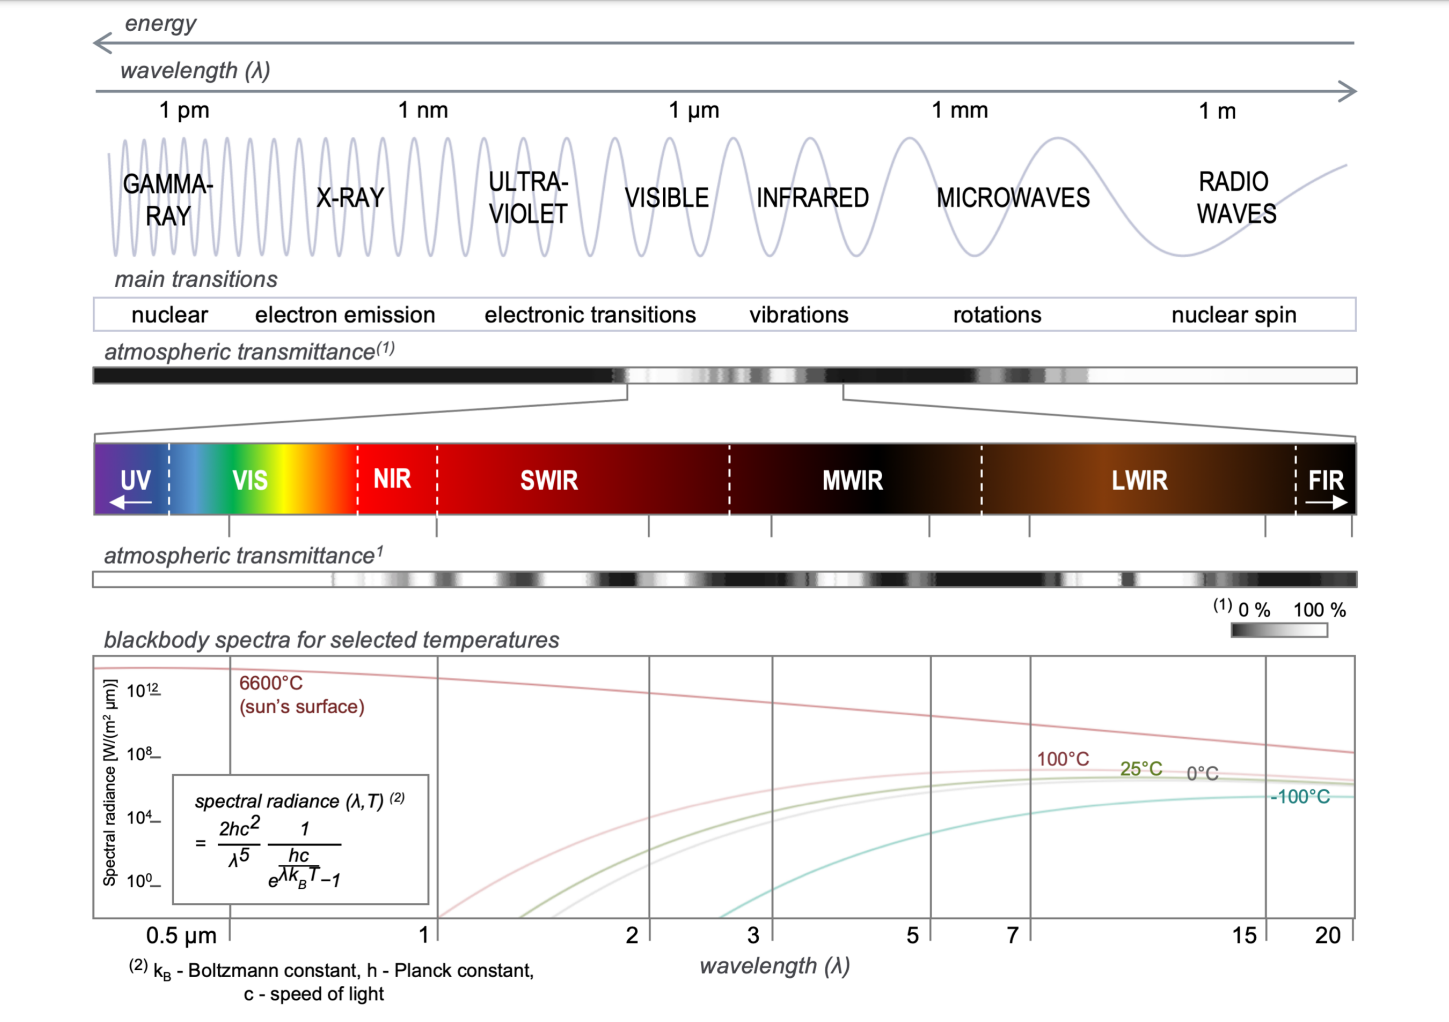
\includegraphics[width=.95\textwidth]{electromagn-spectrum.png}  
	\caption{The electromagnetic spectrum \citep{lorenz2019}}
	\label{fig:em-spec}
\end{figure}

\subsection{Lorem Ipsum 1}
\subsection{Lorem Ipsum 1}
\subsection{Lorem Ipsum 1}
\section{Lorem Ipsum 1}
\subsection{Lorem Ipsum 1}
\subsection{Lorem Ipsum 1}
\section{Lorem Ipsum 1}
\subsection{Lorem Ipsum 1}
\subsubsection{Lorem Ipsum 1}
\section{Lorem Ipsum 1}
\subsection{Lorem Ipsum 1}
\subsection{Lorem Ipsum 1}
\subsubsection{Lorem Ipsum 1}
\section{Lorem Ipsum 1}
\section{Lorem Ipsum 1}

\chapter{PREVIOUS WORKS}

Lorem ipsum dolor sit amet, consectetur adipiscing elit, sed do eiusmod tempor incididunt ut labore et dolore magna aliqua. Amet nulla facilisi morbi tempus iaculis urna id volutpat lacus. Nisl nisi scelerisque eu ultrices vitae auctor. Nisi scelerisque eu ultrices vitae auctor eu augue. Orci sagittis eu volutpat odio. Dolor purus non enim praesent elementum facilisis leo. Ultrices neque ornare aenean euismod. Consectetur libero id faucibus nisl tincidunt. At auctor urna nunc id cursus. Turpis cursus in hac habitasse platea dictumst quisque. Id aliquet risus feugiat in ante metus dictum. Risus viverra adipiscing at in tellus integer feugiat scelerisque. Arcu non odio euismod lacinia at quis risus. Eget magna fermentum iaculis eu non diam phasellus. Cras semper auctor neque vitae tempus quam pellentesque nec. Ultrices gravida dictum fusce ut placerat orci nulla pellentesque dignissim. Massa sapien faucibus et molestie ac feugiat. Magna fringilla urna porttitor rhoncus dolor purus non enim. Amet massa vitae tortor condimentum lacinia quis vel eros. At varius vel pharetra vel turpis nunc eget.

\chapter{METHODOLOGY}
\minitoc 

\section{General methodology}

Table \ref{table:1} is an example of a referenced \LaTeX{} element.

\begin{table}[h!]
\centering
\begin{tabular}{||c c c c||} 
 \hline
 Col1 & Col2 & Col2 & Col3 \\ [0.5ex] 
 \hline\hline
 1 & 6 & 87837 & 787 \\ 
 2 & 7 & 78 & 5415 \\
 3 & 545 & 778 & 7507 \\
 4 & 545 & 18744 & 7560 \\
 5 & 88 & 788 & 6344 \\ [1ex] 
 \hline
\end{tabular}
\caption{Table to test captions and labels.}
\label{table:1}
\end{table}

\subsection{Approach 1}
\subsection{Approach 2}
\subsection{Approach 3}
\section{Equipment}
\subsection{Lorem Ipsum 1}
\subsubsection{Technical specifications}
\subsubsection{Output files}
\subsubsection{Working principle}
\subsection{Lorem Ipsum 1}
\subsection{Lorem Ipsum 2}
\subsection{Lorem Ipsum 3}
\section{Software}
\subsection{Lorem Ipsum 2}
\subsubsection{Lorem Ipsum 2.1}
\subsubsection{Lorem Ipsum 2.2}
\subsubsection{Lorem Ipsum 2.3}
\subsubsection{Lorem Ipsum 2.4}
\subsection{Lorem Ipsum 3}
\subsection{Lorem Ipsum 4}
\subsection{Lorem Ipsum 5}
\chapter{IMPLEMENTATION \& RESULTS}
\minitoc

\section{Lorem Ipsum 0}
\section{Lorem Ipsum 1}
\section{Lorem Ipsum 2}
\section{Lorem Ipsum 3}
\section{Lorem Ipsum 4}
\section{Lorem Ipsum 5}
\section{Lorem Ipsum 6}
\chapter{CONCLUSIONS}

Lorem ipsum dolor sit amet, consectetur adipiscing elit, sed do eiusmod tempor incididunt ut labore et dolore magna aliqua. Amet nulla facilisi morbi tempus iaculis urna id volutpat lacus. Nisl nisi scelerisque eu ultrices vitae auctor. Nisi scelerisque eu ultrices vitae auctor eu augue. Orci sagittis eu volutpat odio. Dolor purus non enim praesent elementum facilisis leo. Ultrices neque ornare aenean euismod. Consectetur libero id faucibus nisl tincidunt. At auctor urna nunc id cursus. Turpis cursus in hac habitasse platea dictumst quisque. Id aliquet risus feugiat in ante metus dictum. Risus viverra adipiscing at in tellus integer feugiat scelerisque. Arcu non odio euismod lacinia at quis risus. Eget magna fermentum iaculis eu non diam phasellus. Cras semper auctor neque vitae tempus quam pellentesque nec. Ultrices gravida dictum fusce ut placerat orci nulla pellentesque dignissim. Massa sapien faucibus et molestie ac feugiat. Magna fringilla urna porttitor rhoncus dolor purus non enim. Amet massa vitae tortor condimentum lacinia quis vel eros. At varius vel pharetra vel turpis nunc eget.
\begin{lstlisting}[language=Python, caption=Code snippet example]
import numpy as np
    
def incmatrix(genl1,genl2):
    m = len(genl1)
    n = len(genl2)
    M = None #to become the incidence matrix
    VT = np.zeros((n*m,1), int)  #dummy variable

    test = "String"
    
    #compute the bitwise xor matrix
    M1 = bitxormatrix(genl1)
    M2 = np.triu(bitxormatrix(genl2),1) 

    for i in range(m-1):
        for j in range(i+1, m):
            [r,c] = np.where(M2 == M1[i,j])
            for k in range(len(r)):
                VT[(i)*n + r[k]] = 1;
                VT[(i)*n + c[k]] = 1;
                VT[(j)*n + r[k]] = 1;
                VT[(j)*n + c[k]] = 1;
                
                if M is None:
                    M = np.copy(VT)
                else:
                    M = np.concatenate((M, VT), 1)
                
                VT = np.zeros((n*m,1), int)
    
    return M
\end{lstlisting}


\lstinputlisting[language=Python,nolol]{./1-mainmatter/test.py}


% column

%\begin{figure}[ht]
%
%	\begin{subfigure}{\textwidth}
%	    \centering
%		\includegraphics[width=.3\textwidth]{mount-nikon-telops.jpg}  
%%	    \caption{img1}
%	    \label{fig:doc1}
%	    \end{subfigure}
%
%	\begin{subfigure}{\textwidth}
%	    \centering
%		\includegraphics[width=.3\textwidth]{mount-nikon-telops1.jpg}  
%	    \caption{img1}
%	    \label{fig:doc1}
%	    \end{subfigure}
%	    
%	\begin{subfigure}{\textwidth}
%	    \centering
%		\includegraphics[width=.3\textwidth]{mount-nikon-telops4.jpg}  
%	    \caption{img1}
%	    \label{fig:doc1}
%	    \end{subfigure}
%	    
%	\caption{Logo IAV}
%	\label{fig:iav}		
%\end{figure}

% --------- Appendices
\begin{appendices}
\includepdfset{pages=-}

\begin{center}
	\vspace*{\stretch{1}}
		 \fontsize{50}{60}\selectfont APPENDICES
	\vspace*{\stretch{1}}
\end{center}
\thispagestyle{empty}
\newpage

\chapter{Camera Mounting System}
\label{appendix:mount-sys}

Lorem ipsum dolor sit amet, consectetur adipiscing elit, sed do eiusmod tempor incididunt ut labore et dolore magna aliqua. Amet nulla facilisi morbi tempus iaculis urna id volutpat lacus. Nisl nisi scelerisque eu ultrices vitae auctor. Nisi scelerisque eu ultrices vitae auctor eu augue. Orci sagittis eu volutpat odio. Dolor purus non enim praesent elementum facilisis leo. Ultrices neque ornare aenean euismod. Consectetur libero id faucibus nisl tincidunt. At auctor urna nunc id cursus. Turpis cursus in hac habitasse platea dictumst quisque. Id aliquet risus feugiat in ante metus dictum. Risus viverra adipiscing at in tellus integer feugiat scelerisque. Arcu non odio euismod lacinia at quis risus. Eget magna fermentum iaculis eu non diam phasellus. Cras semper auctor neque vitae tempus quam pellentesque nec. Ultrices gravida dictum fusce ut placerat orci nulla pellentesque dignissim. Massa sapien faucibus et molestie ac feugiat. Magna fringilla urna porttitor rhoncus dolor purus non enim. Amet massa vitae tortor condimentum lacinia quis vel eros. At varius vel pharetra vel turpis nunc eget.

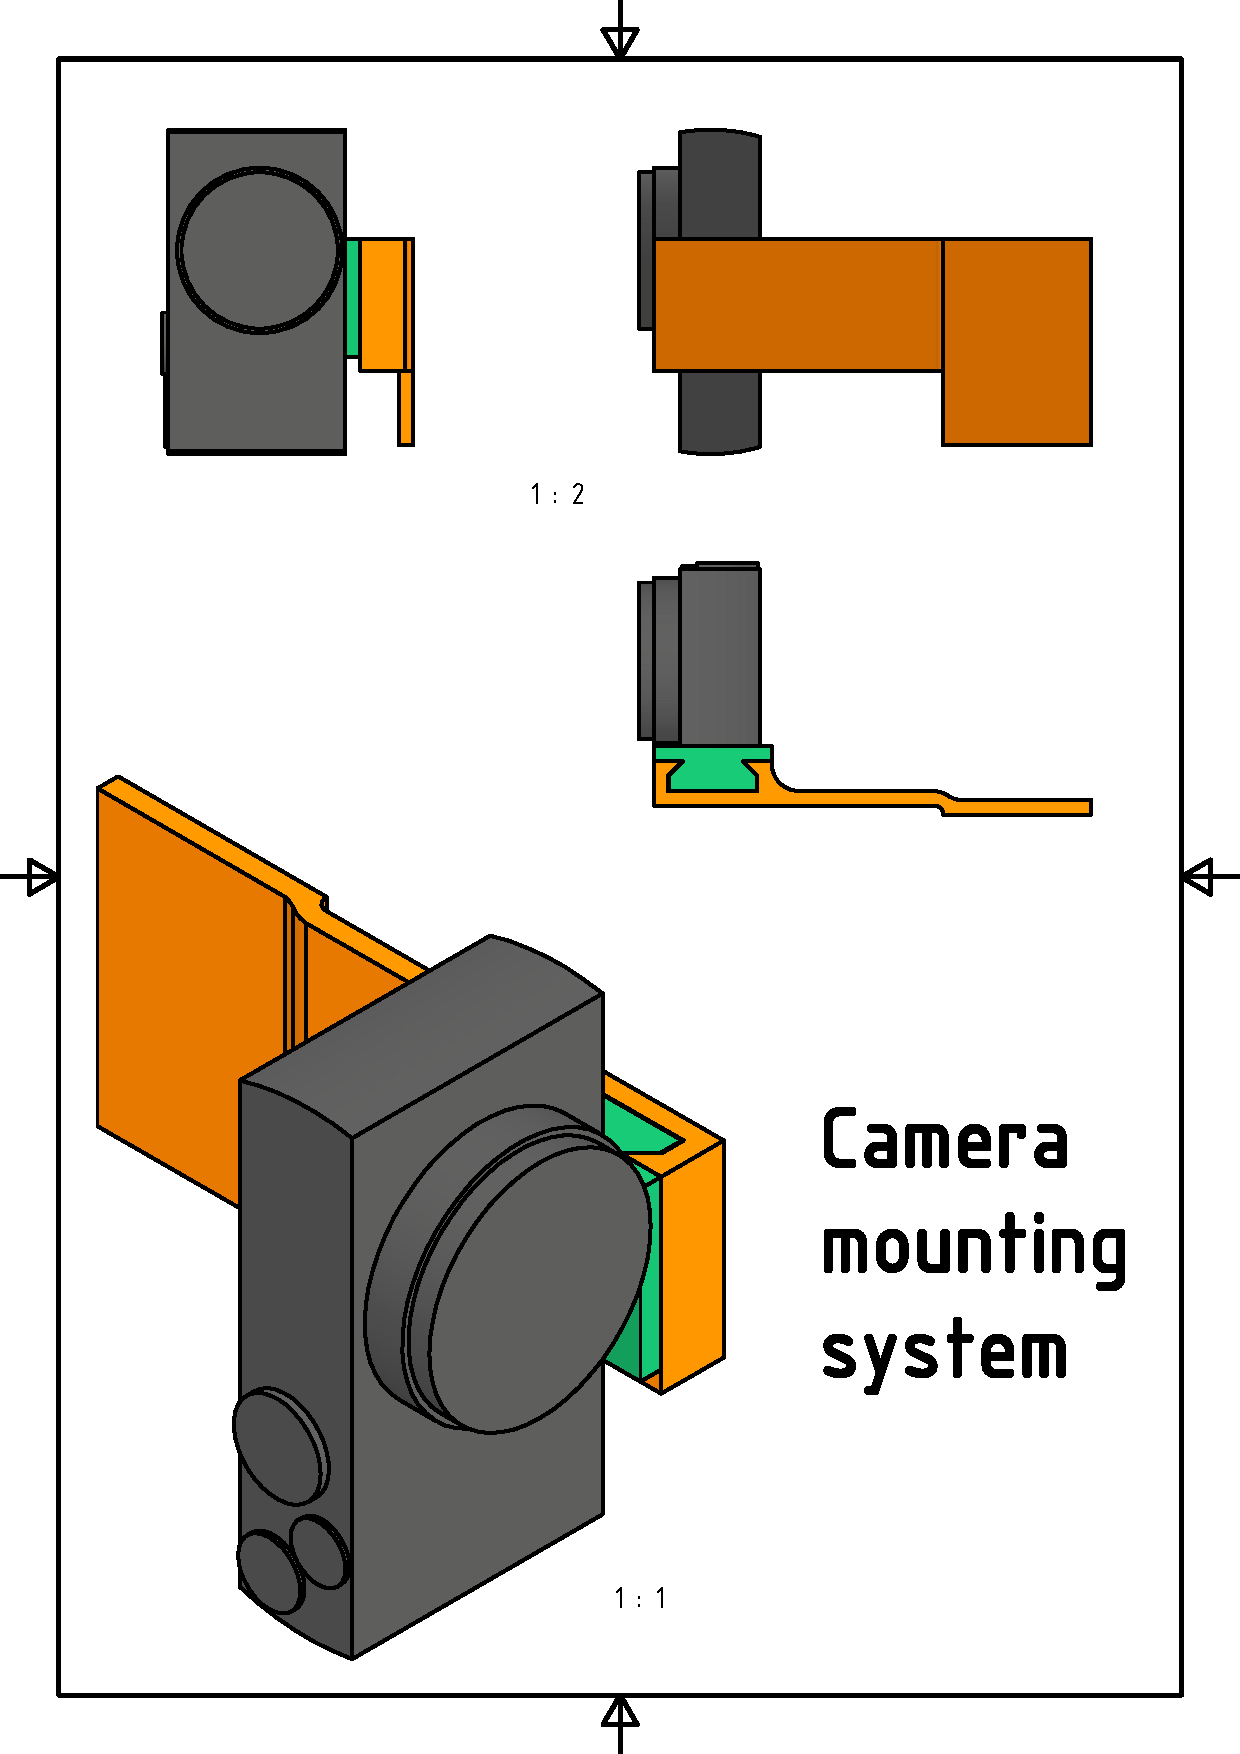
\includepdf{2-appendices/assembly.pdf}

\end{appendices}


\backmatter
\bibliographystyle{apalike}
\phantomsection
\addcontentsline{toc}{chapter}{Bibliography}
\bibliography{3-backmatter/pfe22refs}
% --------- list of acronyms
\chapter{Acronyms}
\begin{acronym}[]  
\acro{RTFM}{Read The Flying Manual}
\end{acronym}

% how to use
% \ac To enter an acronym inside the text
% \acs To get the short version of the acronym, use the command
% \acl Gives you the expanded acronym without even mentioning the acronym
% \acro In the acronym environment, acronyms are defined with the command:
% \acro{acronym}[short name]{full name}
\end{document}
